\subsubsection{Hadron Colliders}
Hadron colliders currently have the advantage over lepton colliders of being highest in energy: with muon colliders a subject of ongoing research and development \cite{Fermi:Muon:Online}, all extant and historical lepton colliders have used beams of electrons, which are many orders of magnitude lighter than the proton. Because $m_{p}\gg m_{e}$, the proton has a higher much rest-mass energy and suffers less from synchrotron losses. Hadron colliders are therefore natural ``energy frontier'' machines, with the Large Hadron Collider the latest and arguably most famous example.

There is however a penalty associated with the use of hadrons: because protons are composite particles, comprising a ``sea'' of quarks and gluons, colliding beams of protons results in collisions between the composite partons. As a result, the energies of the collisions are not well-defined: on average, each quark carries $\frac{1}{3}$ of the energy of the proton; in reality collisions take place over an energy spectrum. Without knowing the initial energies of the colliding particles, it is difficult \textendash if not impossible \textendash to use the principle of conservation of energy to calculate the expected masses of the collision products [\ref{interview:butterworth}]. Since protons also interact via the strong force, the uncertainties in the calculations are higher than for weakly-interacting particles like electrons [\ref{interview:butterworth}]. This means that measurements made at hadron machines are inherently less precise than those made at lepton (and lepton-hadron) machines.
\subsubsection{Tevatron}
The Tevatron was a 6.3km $p\overline{p}$ circular accelerator located at Fermilab in Illinois. Its maximum energy was 1 TeV \textendash hence the name. At the time of its construction in 1983, this was the man-made energy frontier. To date, the Tevatron is the second-highest energy machine ever built, surpassed only by the Large Hadron Collider.

\begin{figure}[!htb]
\centering
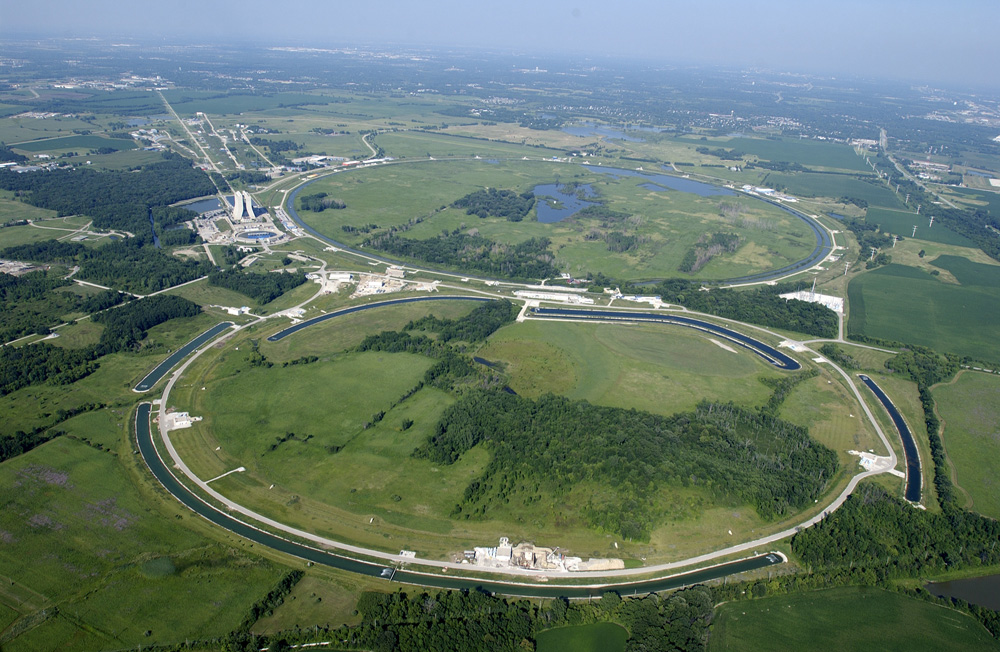
\includegraphics[width=0.7\textwidth,natwidth=1000,natheight=652]{fermilabaccleratorcomplex.jpg}
\caption{Fermilab's Accelerator Complex \cite{Tevatron:Antiprotons:Online}}
\end{figure}

The Tevatron was proposed as a replacement for Fermilab's 500 GeV Main Ring accelerator, which was based on room-temperature electromagnets, and required the development of high-quality superconducting magnets to accelerate the beam, and the design and construction of an antiproton source \cite{Tevatron:Retrospective:Online}. The use of antiprotons allowed the Tevatron to circulate both beams within the same magnet ring (due to the reversed charge on the antiproton), thus saving infrastructure and engineering costs; however, a major limitation to the luminosity of the machine, and therefore the primary focus for upgrades, was the production of antiprotons. The antiprotons used in the Tevatron were produced by ``smashing'' protons into a nickel target, yielding about 20 antiprotons for every $10^{9}$ protons collided with the target \cite{Tevatron:Antiprotons:Online}.

In 1995, the CDF and D\O$\:$ experiments announced the discovery of the top quark, the last fundamental fermion predicted by the Standard Model, with a certainty of 99.9998\% \cite{PhysRevLett:Top1,PhysRevLett:Top2}. Before the completion of the Large Hadron Collider, the Tevatron was the only particle collider energetic enough to produce top quarks. Other discoveries incuded observations of two types of $\sigma$ baryons \cite{Fermi:Sigma:Online}, a $\Xi_{b}^{-}$ baryon \cite{Fermi:Xi:Online}, and a ``double strange'' $\Omega_{b}^{-}$ baryon \cite{PhysRevLett:Omega}. On 2nd July 2012 scientists from the CDF and D\O\: collaborations announced data in support of the existence of a Higgs boson with a mass in the region of 115 to 135 GeV \cite{Fermi:Higgs:Online}; two days later scientists from the LHC announced the discovery of a Higgs with a mass of 125.3 $\pm$ 0.4 (CMS) GeV \cite{PhysLettB:Higgs:CMS} or 126 $\pm$ 0.4 (ATLAS) GeV \cite{PhysLettB:Higgs:ATLAS} \textendash frustratingly, the Higgs boson was so close to the top of the Tevatron's energy range that the Tevatron alone could not furnish proof of its existence.

\subsubsection{Superconducting Super Collider (SSC)}
The Superconducting Super Collider was a proposed proton-proton \cite{SSC:LAT:Online} collider to be built in Texas with a 87.1 km ring circumference. This would have yielded an energy of 20 TeV per proton, and a centre-of-mass-energy of 40 TeV. By comparison, when the Large Hadron Collider reopens in 2015, it will be colliding beams at a centre-of-mass-energy of 13 TeV \cite{LHC:14TeV:Online}. Over 20km worth of tunnel had been excavated and 2,000 on-site staff lost their jobs when the project was cancelled \cite{SSC:Sun:Online}.

\begin{figure}[!htb]
\centering
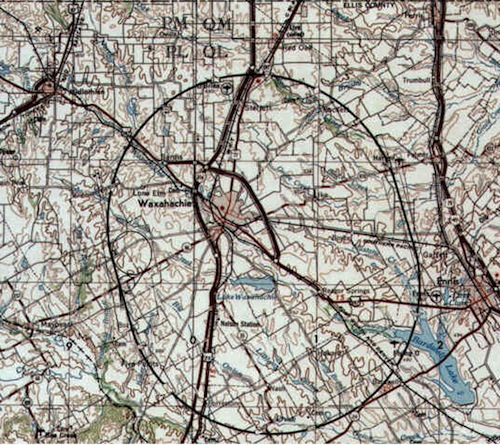
\includegraphics[width=0.7\textwidth,natwidth=500,natheight=445]{sscmap.jpg}
\caption{The SSC was to encircle the town of Waxahachie, Texas \cite{SSC:SI:Online}}
\end{figure}

The reasons for the failure of the Superconducting Super Collider project are many, complex and varied: ultimately budgetary concerns were cited as the reason for cancellation \textendash the United States Congress approved a budget of \$4.4 billion \cite{SSC:BE} for the project in 1987, but cost estimates blew up to over \$11 billion \cite{SSC:LAT:Online} after construction started \textendash however, in large part the project was smothered in its cradle by politics. Prof Steven Weinberg writes:

\begin{quote}
Projected costs did increase, but the main reason was that, year by year, Congress never supplied sufficient funds to keep to the planned rate of spending. This stretched out the time and hence the cost to complete the project. Even so, the SSC met all technical challenges, and could have been completed for about what has been spent on the LHC, and completed a decade earlier. \cite{SSC:Weinberg:Online}
\end{quote}

Prof Jon Butterworth also stated that, ``You can't have it both ways. You've got to either do it as a national project, where you have some helpers, [...] or you do something like CERN where there's no one country in control,'' adding that the decision about whether to fund the International Linear Collider (ILC) as a national prestige project or a collaboration was key to the success of the project [\ref{interview:butterworth}]. The Superconducting Super Collider serves as a cautionary tale about the need for strong political support, and a clear revenue stream.

\subsubsection{Relativistic Heavy Ion Collider (RHIC)}
The Relativistic Heavy Ion Collider (RHIC) is an intersecting storage ring particle accelerator located at the Brookhaven National Laboratory in New York; along with the Large Hadron Collider, which collides ions for one month of the year, it is one of two operational heavy-ion colliders. It is the only spin-polarised proton collider ever built \cite{RHIC:Spin}, which enables it to perform experiments on the spin structure of the proton.

Since the spins of the proton's quarks account for less than one third of its overall spin \cite{PhysLettB:ProtonSpin}, the ``proton spin crisis'' is an important unresolved question in quantum chromodynamics \textendash with potential ramifications for technologies such as Magnetic Resonance Imaging (MRI) \textendash which can be probed by this machine. Notably, the scientists at the RHIC have ``tentatively'' claimed to have created a quark-gluon plasma \cite{NucPhysA:QuarkGluon} \textendash a hypothetical phase of QCD supposed to have existed in the early universe \cite{CERN:QuarkGluonPlasma:Online}. The obvious drawback of the RHIC relative to the LHC is its lower energy \textendash up to around 200 GeV for Au + Au collisions; however, since it runs a dedicated heavy-ion collision programme it outputs more data on the subject compared to the LHC, which collides ions for one month of the year.

\subsubsection{Large Hadron Collider (LHC)}
At 27km in circumference and boasting a centre-of-mass-energy of up to 13 TeV \cite{LHC:14TeV:Online,CERN:14TeV:Online}, the Large Hadron Collider is the largest and most energetic particle collider ever built \cite{LHC:Home}. Located at CERN in Geneva, Switzerland, and crossing the Franco-Swiss border, the Large Hadron Collider is considered ``one of the great engineering milestones of mankind'' \cite{LHC:Milestone:Online}. To date, the great success of the Large Hadron Collider project, and primary reason for funding it, was the discovery of a Higgs boson in 2012 \cite{PhysLettB:Higgs:ATLAS,PhysLettB:Higgs:CMS}. Additionally, the LHC has reported the creation of a quark-gluon plasma \cite{NatGeo:QuarkGluon:Online}, observed the $\chi_{b}$(3P) bottomonium state \cite{arXiv:ATLAS:Bottomonium}, and observed a very rare ($B_{s}^{0} \rightarrow \mu^{+}\mu^{-}$) decay which puts constraints on the likelihood of supersymmetry being correct \cite{BBC:SUSY}. An accident at the LHC in 2008, which involved an electrical fault leading to six tonnes of liquid helium venting into the tunnel and causing an explosion, flags up the importance of stringent failsafes in large-scale experiments. \cite{BBC:MagnetQuench:Online} According to CERN's interim report on the incident: ``Proper safety procedures were in force, safety 
systems performed as expected, and no one was put at risk,'' but the faulty electrics caused an electric arc, which resulted in the explosion \cite{CERN:IncidentReport}.

\begin{figure}[!htb]
\centering
\includegraphics[width=0.7\textwidth,natwidth=1200,natheight=1081]{lhc.jpg}
\caption{The scale of the LHC \cite{ATLAS:Gallery:Online}}
\end{figure}

Due to the low efficiency in the manufacture of antiprotons, the Large Hadron Collider uses colliding beams of protons. The LHC produces data at a rate of tens of petabytes (tens of millions of gigabytes) per year, requiring \textendash by 2012 \textendash the world's largest computer grid, ``a global collaboration of computing centres in nearly 40 countries'', to analyse \cite{LHC:ComputingGrid:Online}.

The Large Hadron Collider is a shining example of the kind of success a well-planned and well-funded large-scale project can achieve; however, it is worth remembering, as Prof Jon Butterworth noted, that ``there was an absolutely first-class science case for the LHC,'' \textendash in other words: it was clear that the Large Hadron Collider was either going to prove or disprove the existence of a Standard Model Higgs, which theoretically had to exist within the energy range accessible at the LHC. This was a clear aim for the project from the outset. However, the lack of additional discoveries \textendash such as supersymmetric particles and dark matter candidates \textendash casts a shadow of doubt over the utility of pushing back the energy barrier further without the theoretical framework to put an upper limit on the mass estimates of these hypothetical particles [\ref{interview:butterworth}]. Additionally, the Large Hadron Collider elided some of the civil engineering costs associated with large particle collider projects because it was built in a pre-existing tunnel (which had previously housed the electron-position collider, LEP) \cite{CERN:LEP:Online}.

\subsubsection{Lepton Colliders}
At present, the only realistic design for a lepton collider utilises beams of electrons (and positrons). The obvious drawback is the small mass of the electron, which places a limit on how energetic the beam can be \textendash particularly for circular colliders, which suffer synchrotron losses. Future designs might use heavier muon or tau particles \cite{Fermi:Muon:Online}, raising the energy ranges available with these colliders.

The particular advantage of a lepton collider is the degree of precision to which measurements can be made, both because leptons are fundamental particles \textendash so the energies of the collisions are well-defined \textendash and because electrons are not subject to the strong force, so the theoretical calculations are also more precise [\ref{interview:thorne}].

\subsubsection{Large Electron-Positron Collider (LEP)}
The Large Electron-Positron Collider, the previous inhabitant of the Large Hadron Collider's 27 km tunnel, was and remains the largest lepton collider ever built. It was completed in 1988, and reached a peak centre-of-mass-energy of 209 GeV \cite{CERN:LEP:Online}. The primary focus of LEP was on measuring the electroweak interaction, and particularly determining the masses of the W and Z bosons, which had been discovered in 1983 (although the most precise measurement of the W mass actually comes from the Tevatron [\ref{interview:butterworth}]). The civil engineering costs associated with building LEP accounted for over half of the construction budget for the machine \cite{LEP:History:Online}. In addition to producing hundreds of thousands of Z bosons \cite{LEP:History:Online}, the machine measured the strength of the strong interaction as decreasing with energy in agreement with quantum chromodynamic theory, and determined the number of particle families with light neutrinos as $2.982\pm 0.013$, in agreement with the Standard Model prediction of 3 \cite{ALEPH:Physics:Online}.

\subsubsection{Lepton-Hadron Colliders}
Lepton-hadron colliders are a``best (and worst) of both worlds'' approach. The use of hadrons means that they can reach higher energies than lepton-only colliders, and the use of leptons means a higher degree of precision than hadron-only colliders. They are particularly good at probing the structure of the proton, and studying quantum chromodynamics (the strong interaction) [\ref{interview:waters}, \ref{interview:thorne}, \ref{interview:butterworth}]. However, they are less energetic than hadron-only machines, and less precise than lepton-only machines.

\subsubsection{Hadron-Elektron Ringanglage (HERA)}
HERA was a 6.3 km particle accelerator located at the Deutsches Elektronen-Synchrotron (DESY) research centre in Hamburg. It collided electrons and positrons with protons at a centre-of-mass-energy of 318 GeV from 1992 to 2007 \cite{PHYS:HERA}. The data obtained at HERA allowed experimenters to obtain the individual parton distribution functions describing the composite nature of the proton and gave ``no indication of a quark substructure down to a scale order of $10^{-18}$m'' \cite{SPS:HERA}, providing strong evidence for the fundamental nature of quarks. HERA measurements also ``confirmed the nature of the strong force as it was predicted by physicists David Gross, David Politzer, and Frank Wilczek'' \cite{PHYS:HERA}. The HERA experiment has been very successful in probing the structure of the proton and testing theoretical models of the strong force; however, any future lepton-hadron collider would necessarily focus on the same area without providing much opportunity to make the kinds of precision measurements available to lepton-only colliders, or push back the energy frontier like a hadron-only collider.
